\subsection{Project Block Diagram}

\noindent As indicated by color and work breakdown delegation, the three subsystems of obstacle detection, identification, and avoidance are shown. The peripherals, depicted in the diagram by circles, are functionally sensors and feedback for user guidance. \\

\noindent The microcontroller unit is central to system integration. It will receive and transmit data from the peripherals while also communicating with the motor controller to steer and drive. In turn, the position determination algorithm, coupled with the speed and steering control, comprise the object avoidance function. Computer vision and image processing are also encompassed by this obstacle identification subsystem. Headlights are an optional advanced requirement feature configured to turn on in lowlight environments. Finally, an implicit element of the diagram are the power inputs from the battery supply.\\

\noindent As seen below, each of the team members will be taking a lead role for different subsystems of the project. These roles were divided based on individual interests and skills, seeking to maximize overall productivity and effectiveness for the designs specified.\\

\noindent Tobiah, being an electrical engineering student with a focus in signal processing, will be covering the obstacle detection subsystem. This will involve research regarding the sensors and generating the range solution. The task at hand is then to give the walker vision of its surroundings without using cameras or any form of pre-planned pathing. FORWARD should be a reactive guidance system. \\

\noindent Morgan, being an electrical engineer interested in robotics and power, will be covering all subsystems under those categories. This includes the power supply as well as the more electromechanical components of the project such as the motors, headlights, and haptic feedback. The power supply will need to provide energy both to the MCU and to the different outputs. The MCU will then control these outputs, the headlights directly through the MCU and the motors for the wheels and haptic feedback using a motor controller. This will allow the system to functionally turn and avoid obstacles as well as vibrate to alert the user of obstacles. \\

\noindent As depicted by the blue shading, Matthew will be taking lead over most of the software related subsystems as well as the MCU. Since the camera will be primarily involved in transmitting video to the MCU for AI image processing – Matthew will be responsible for selecting the camera. The Audio Feedback Guidance will also involve heavy software support since it will be over Bluetooth, so this is also within Matthew’s scope. The MCU will drive everything, facilitating all communication through embedded programming and so it is also within Matthew’s scope.

\begin{figure}[H]
	\centering
	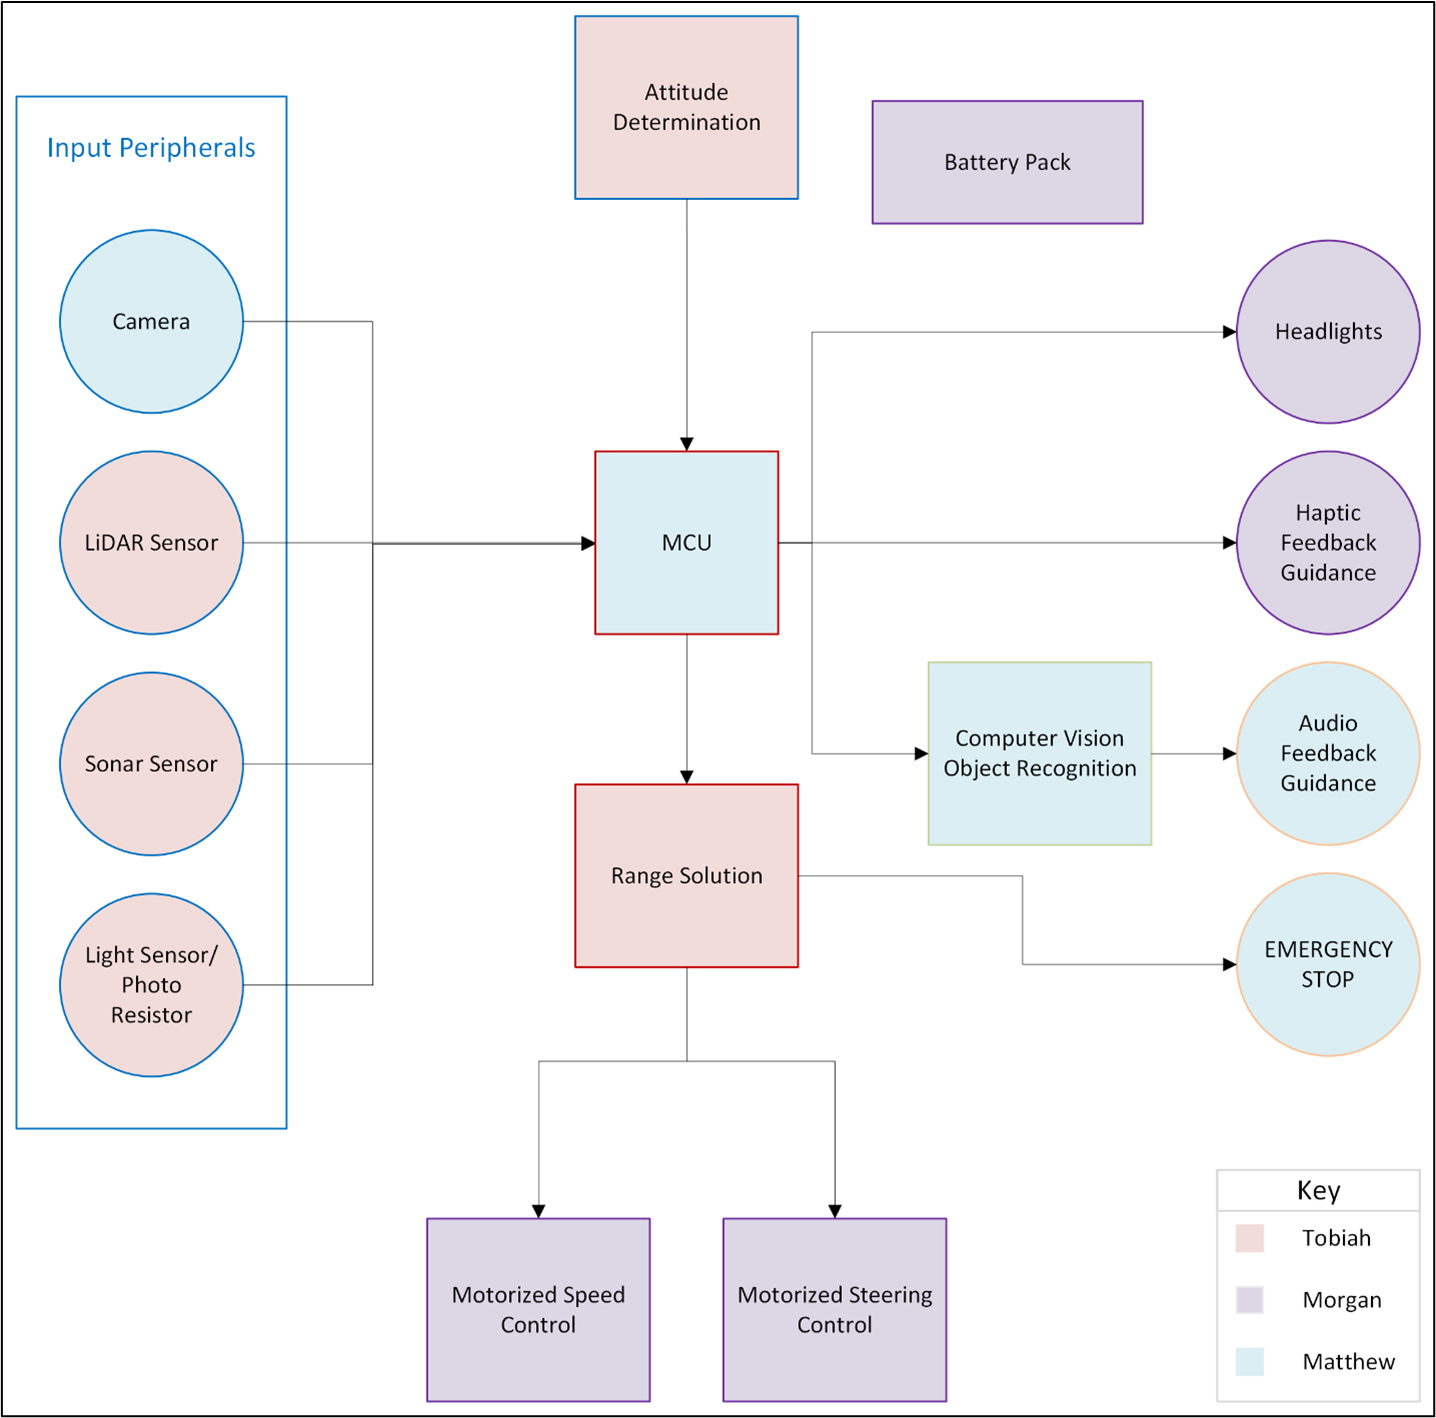
\includegraphics[width=0.95\textwidth]{./Images/AbstractSysBlk.png}
	\caption{\label{fig:AbstractSysBlk}System Block Diagram}
\end{figure}
